
%% bare_jrnl.tex
%% V1.4b
%% 2015/08/26
%% by Michael Shell
%% see http://www.michaelshell.org/
%% for current contact information.
%%
%% This is a skeleton file demonstrating the use of IEEEtran.cls
%% (requires IEEEtran.cls version 1.8b or later) with an IEEE
%% journal paper.
%%
%% Support sites:
%% http://www.michaelshell.org/tex/ieeetran/
%% http://www.ctan.org/pkg/ieeetran
%% and
%% http://www.ieee.org/

%%*************************************************************************
%% Legal Notice:
%% This code is offered as-is without any warranty either expressed or
%% implied; without even the implied warranty of MERCHANTABILITY or
%% FITNESS FOR A PARTICULAR PURPOSE! 
%% User assumes all risk.
%% In no event shall the IEEE or any contributor to this code be liable for
%% any damages or losses, including, but not limited to, incidental,
%% consequential, or any other damages, resulting from the use or misuse
%% of any information contained here.
%%
%% All comments are the opinions of their respective authors and are not
%% necessarily endorsed by the IEEE.
%%
%% This work is distributed under the LaTeX Project Public License (LPPL)
%% ( http://www.latex-project.org/ ) version 1.3, and may be freely used,
%% distributed and modified. A copy of the LPPL, version 1.3, is included
%% in the base LaTeX documentation of all distributions of LaTeX released
%% 2003/12/01 or later.
%% Retain all contribution notices and credits.
%% ** Modified files should be clearly indicated as such, including  **
%% ** renaming them and changing author support contact information. **
%%*************************************************************************


% *** Authors should verify (and, if needed, correct) their LaTeX system  ***
% *** with the testflow diagnostic prior to trusting their LaTeX platform ***
% *** with production work. The IEEE's font choices and paper sizes can   ***
% *** trigger bugs that do not appear when using other class files.       ***                          ***
% The testflow support page is at:
% http://www.michaelshell.org/tex/testflow/



\documentclass[journal]{IEEEtran}
%
% If IEEEtran.cls has not been installed into the LaTeX system files,
% manually specify the path to it like:
% \documentclass[journal]{../sty/IEEEtran}





% Some very useful LaTeX packages include:
% (uncomment the ones you want to load)


% *** MISC UTILITY PACKAGES ***
%
%\usepackage{ifpdf}
% Heiko Oberdiek's ifpdf.sty is very useful if you need conditional
% compilation based on whether the output is pdf or dvi.
% usage:
% \ifpdf
%   % pdf code
% \else
%   % dvi code
% \fi
% The latest version of ifpdf.sty can be obtained from:
% http://www.ctan.org/pkg/ifpdf
% Also, note that IEEEtran.cls V1.7 and later provides a builtin
% \ifCLASSINFOpdf conditional that works the same way.
% When switching from latex to pdflatex and vice-versa, the compiler may
% have to be run twice to clear warning/error messages.






% *** CITATION PACKAGES ***
%
\usepackage{cite}
% cite.sty was written by Donald Arseneau
% V1.6 and later of IEEEtran pre-defines the format of the cite.sty package
% \cite{} output to follow that of the IEEE. Loading the cite package will
% result in citation numbers being automatically sorted and properly
% "compressed/ranged". e.g., [1], [9], [2], [7], [5], [6] without using
% cite.sty will become [1], [2], [5]--[7], [9] using cite.sty. cite.sty's
% \cite will automatically add leading space, if needed. Use cite.sty's
% noadjust option (cite.sty V3.8 and later) if you want to turn this off
% such as if a citation ever needs to be enclosed in parenthesis.
% cite.sty is already installed on most LaTeX systems. Be sure and use
% version 5.0 (2009-03-20) and later if using hyperref.sty.
% The latest version can be obtained at:
% http://www.ctan.org/pkg/cite
% The documentation is contained in the cite.sty file itself.






% *** GRAPHICS RELATED PACKAGES ***
%
\ifCLASSINFOpdf
  \usepackage[pdftex]{graphicx}
  % declare the path(s) where your graphic files are
  \graphicspath{{./pics/}}
  % and their extensions so you won't have to specify these with
  % every instance of \includegraphics
  \DeclareGraphicsExtensions{.pdf,.jpeg,.png}
\else
  % or other class option (dvipsone, dvipdf, if not using dvips). graphicx
  % will default to the driver specified in the system graphics.cfg if no
  % driver is specified.
  \usepackage[dvips]{graphicx}
  % declare the path(s) where your graphic files are
  \graphicspath{{./pics/}}
  % and their extensions so you won't have to specify these with
  % every instance of \includegraphics
  \DeclareGraphicsExtensions{.eps}
\fi
% graphicx was written by David Carlisle and Sebastian Rahtz. It is
% required if you want graphics, photos, etc. graphicx.sty is already
% installed on most LaTeX systems. The latest version and documentation
% can be obtained at: 
% http://www.ctan.org/pkg/graphicx
% Another good source of documentation is "Using Imported Graphics in
% LaTeX2e" by Keith Reckdahl which can be found at:
% http://www.ctan.org/pkg/epslatex
%
% latex, and pdflatex in dvi mode, support graphics in encapsulated
% postscript (.eps) format. pdflatex in pdf mode supports graphics
% in .pdf, .jpeg, .png and .mps (metapost) formats. Users should ensure
% that all non-photo figures use a vector format (.eps, .pdf, .mps) and
% not a bitmapped formats (.jpeg, .png). The IEEE frowns on bitmapped formats
% which can result in "jaggedy"/blurry rendering of lines and letters as
% well as large increases in file sizes.
%
% You can find documentation about the pdfTeX application at:
% http://www.tug.org/applications/pdftex





% *** MATH PACKAGES ***
%
\usepackage{amsmath}
% A popular package from the American Mathematical Society that provides
% many useful and powerful commands for dealing with mathematics.
%
% Note that the amsmath package sets \interdisplaylinepenalty to 10000
% thus preventing page breaks from occurring within multiline equations. Use:
%\interdisplaylinepenalty=2500
% after loading amsmath to restore such page breaks as IEEEtran.cls normally
% does. amsmath.sty is already installed on most LaTeX systems. The latest
% version and documentation can be obtained at:
% http://www.ctan.org/pkg/amsmath





% *** SPECIALIZED LIST PACKAGES ***
%
%\usepackage{algorithmic}
% algorithmic.sty was written by Peter Williams and Rogerio Brito.
% This package provides an algorithmic environment fo describing algorithms.
% You can use the algorithmic environment in-text or within a figure
% environment to provide for a floating algorithm. Do NOT use the algorithm
% floating environment provided by algorithm.sty (by the same authors) or
% algorithm2e.sty (by Christophe Fiorio) as the IEEE does not use dedicated
% algorithm float types and packages that provide these will not provide
% correct IEEE style captions. The latest version and documentation of
% algorithmic.sty can be obtained at:
% http://www.ctan.org/pkg/algorithms
% Also of interest may be the (relatively newer and more customizable)
% algorithmicx.sty package by Szasz Janos:
% http://www.ctan.org/pkg/algorithmicx




% *** ALIGNMENT PACKAGES ***
%
%\usepackage{array}
% Frank Mittelbach's and David Carlisle's array.sty patches and improves
% the standard LaTeX2e array and tabular environments to provide better
% appearance and additional user controls. As the default LaTeX2e table
% generation code is lacking to the point of almost being broken with
% respect to the quality of the end results, all users are strongly
% advised to use an enhanced (at the very least that provided by array.sty)
% set of table tools. array.sty is already installed on most systems. The
% latest version and documentation can be obtained at:
% http://www.ctan.org/pkg/array


% IEEEtran contains the IEEEeqnarray family of commands that can be used to
% generate multiline equations as well as matrices, tables, etc., of high
% quality.




% *** SUBFIGURE PACKAGES ***
%\ifCLASSOPTIONcompsoc
%  \usepackage[caption=false,font=normalsize,labelfont=sf,textfont=sf]{subfig}
%\else
%  \usepackage[caption=false,font=footnotesize]{subfig}
%\fi
% subfig.sty, written by Steven Douglas Cochran, is the modern replacement
% for subfigure.sty, the latter of which is no longer maintained and is
% incompatible with some LaTeX packages including fixltx2e. However,
% subfig.sty requires and automatically loads Axel Sommerfeldt's caption.sty
% which will override IEEEtran.cls' handling of captions and this will result
% in non-IEEE style figure/table captions. To prevent this problem, be sure
% and invoke subfig.sty's "caption=false" package option (available since
% subfig.sty version 1.3, 2005/06/28) as this is will preserve IEEEtran.cls
% handling of captions.
% Note that the Computer Society format requires a larger sans serif font
% than the serif footnote size font used in traditional IEEE formatting
% and thus the need to invoke different subfig.sty package options depending
% on whether compsoc mode has been enabled.
%
% The latest version and documentation of subfig.sty can be obtained at:
% http://www.ctan.org/pkg/subfig




% *** FLOAT PACKAGES ***
%
%\usepackage{fixltx2e}
% fixltx2e, the successor to the earlier fix2col.sty, was written by
% Frank Mittelbach and David Carlisle. This package corrects a few problems
% in the LaTeX2e kernel, the most notable of which is that in current
% LaTeX2e releases, the ordering of single and double column floats is not
% guaranteed to be preserved. Thus, an unpatched LaTeX2e can allow a
% single column figure to be placed prior to an earlier double column
% figure.
% Be aware that LaTeX2e kernels dated 2015 and later have fixltx2e.sty's
% corrections already built into the system in which case a warning will
% be issued if an attempt is made to load fixltx2e.sty as it is no longer
% needed.
% The latest version and documentation can be found at:
% http://www.ctan.org/pkg/fixltx2e


%\usepackage{stfloats}
% stfloats.sty was written by Sigitas Tolusis. This package gives LaTeX2e
% the ability to do double column floats at the bottom of the page as well
% as the top. (e.g., "\begin{figure*}[!b]" is not normally possible in
% LaTeX2e). It also provides a command:
%\fnbelowfloat
% to enable the placement of footnotes below bottom floats (the standard
% LaTeX2e kernel puts them above bottom floats). This is an invasive package
% which rewrites many portions of the LaTeX2e float routines. It may not work
% with other packages that modify the LaTeX2e float routines. The latest
% version and documentation can be obtained at:
% http://www.ctan.org/pkg/stfloats
% Do not use the stfloats baselinefloat ability as the IEEE does not allow
% \baselineskip to stretch. Authors submitting work to the IEEE should note
% that the IEEE rarely uses double column equations and that authors should try
% to avoid such use. Do not be tempted to use the cuted.sty or midfloat.sty
% packages (also by Sigitas Tolusis) as the IEEE does not format its papers in
% such ways.
% Do not attempt to use stfloats with fixltx2e as they are incompatible.
% Instead, use Morten Hogholm'a dblfloatfix which combines the features
% of both fixltx2e and stfloats:
%
% \usepackage{dblfloatfix}
% The latest version can be found at:
% http://www.ctan.org/pkg/dblfloatfix




%\ifCLASSOPTIONcaptionsoff
%  \usepackage[nomarkers]{endfloat}
% \let\MYoriglatexcaption\caption
% \renewcommand{\caption}[2][\relax]{\MYoriglatexcaption[#2]{#2}}
%\fi
% endfloat.sty was written by James Darrell McCauley, Jeff Goldberg and 
% Axel Sommerfeldt. This package may be useful when used in conjunction with 
% IEEEtran.cls'  captionsoff option. Some IEEE journals/societies require that
% submissions have lists of figures/tables at the end of the paper and that
% figures/tables without any captions are placed on a page by themselves at
% the end of the document. If needed, the draftcls IEEEtran class option or
% \CLASSINPUTbaselinestretch interface can be used to increase the line
% spacing as well. Be sure and use the nomarkers option of endfloat to
% prevent endfloat from "marking" where the figures would have been placed
% in the text. The two hack lines of code above are a slight modification of
% that suggested by in the endfloat docs (section 8.4.1) to ensure that
% the full captions always appear in the list of figures/tables - even if
% the user used the short optional argument of \caption[]{}.
% IEEE papers do not typically make use of \caption[]'s optional argument,
% so this should not be an issue. A similar trick can be used to disable
% captions of packages such as subfig.sty that lack options to turn off
% the subcaptions:
% For subfig.sty:
% \let\MYorigsubfloat\subfloat
% \renewcommand{\subfloat}[2][\relax]{\MYorigsubfloat[]{#2}}
% However, the above trick will not work if both optional arguments of
% the \subfloat command are used. Furthermore, there needs to be a
% description of each subfigure *somewhere* and endfloat does not add
% subfigure captions to its list of figures. Thus, the best approach is to
% avoid the use of subfigure captions (many IEEE journals avoid them anyway)
% and instead reference/explain all the subfigures within the main caption.
% The latest version of endfloat.sty and its documentation can obtained at:
% http://www.ctan.org/pkg/endfloat
%
% The IEEEtran \ifCLASSOPTIONcaptionsoff conditional can also be used
% later in the document, say, to conditionally put the References on a 
% page by themselves.




% *** PDF, URL AND HYPERLINK PACKAGES ***
%
%\usepackage{url}
% url.sty was written by Donald Arseneau. It provides better support for
% handling and breaking URLs. url.sty is already installed on most LaTeX
% systems. The latest version and documentation can be obtained at:
% http://www.ctan.org/pkg/url
% Basically, \url{my_url_here}.




% *** Do not adjust lengths that control margins, column widths, etc. ***
% *** Do not use packages that alter fonts (such as pslatex).         ***
% There should be no need to do such things with IEEEtran.cls V1.6 and later.
% (Unless specifically asked to do so by the journal or conference you plan
% to submit to, of course. )


% correct bad hyphenation here
\hyphenation{op-tical net-works semi-conduc-tor}

\usepackage{color}
\usepackage{amsfonts,amssymb}
\usepackage{soul}

\newcommand{\mauricio}[1]{{\color{blue}#1}}

\newcommand{\simo}[1]{{\color{red}#1}}

\begin{document}
%
% paper title
% can use linebreaks \\ within to get better formatting as desired
% Do not put math or special symbols in the title.
%\title{Latent force models for signal processing and machine learning }
\title{Combining First-Principles and Non-Parametric Statistical Models via Latent Force Models}

%
%
% author names and IEEE memberships
% note positions of commas and nonbreaking spaces ( ~ ) LaTeX will not break
% a structure at a ~ so this keeps an author's name from being broken across
% two lines.
% use \thanks{} to gain access to the first footnote area
% a separate \thanks must be used for each paragraph as LaTeX2e's \thanks
% was not built to handle multiple paragraphs
%

\author{Simo~S\"arkk\"a,~\IEEEmembership{Senior Member,~IEEE,}
        Mauricio~A.~\'Alvarez, 
        and~Neil~D.~Lawrence% <-this % stops a space
\thanks{Simo~S\"arkk\"a is with the Department of Electrical Engineering and Automation (EEA), Aalto University, Rakentajanaukio 2, 02150 Espoo, Finland (simo.sarkka@aalto.fi).}% <-this % stops a space
\thanks{Mauricio A. \'Alvarez is with the Department of Electrical Engineering,
Universidad Tecnol\'ogica de Pereira, Colombia, 660003.}% <-this % stops a space
\thanks{Neil D. Lawrence is with the Department of Computer Science, University of Sheffield,
Sheffield, UK S1 4DP and with The Sheffield Institute for Translational Neuroscience,
Sheffield, UK S10 2HQ.}% <-this % stops a space
\thanks{Manuscript received XXX; revised XXX.}}


% note the % following the last \IEEEmembership and also \thanks -
% these prevent an unwanted space from occurring between the last author name
% and the end of the author line. i.e., if you had this:
%
% \author{....lastname \thanks{...} \thanks{...} }
%                     ^------------^------------^----Do not want these spaces!
%
% a space would be appended to the last name and could cause every name on that
% line to be shifted left slightly. This is one of those "LaTeX things". For
% instance, "\textbf{A} \textbf{B}" will typeset as "A B" not "AB". To get
% "AB" then you have to do: "\textbf{A}\textbf{B}"
% \thanks is no different in this regard, so shield the last } of each \thanks
% that ends a line with a % and do not let a space in before the next \thanks.
% Spaces after \IEEEmembership other than the last one are OK (and needed) as
% you are supposed to have spaces between the names. For what it is worth,
% this is a minor point as most people would not even notice if the said evil
% space somehow managed to creep in.



% The paper headers
\markboth{Journal of \LaTeX\ Class Files,~Vol.~X, No.~X, Month~20XX}%
{Shell \MakeLowercase{\textit{et al.}}: Bare Demo of IEEEtran.cls for Journals}
% The only time the second header will appear is for the odd numbered pages
% after the title page when using the twoside option.
%
% *** Note that you probably will NOT want to include the author's ***
% *** name in the headers of peer review papers.                   ***
% You can use \ifCLASSOPTIONpeerreview for conditional compilation here if
% you desire.




% If you want to put a publisher's ID mark on the page you can do it like
% this:
%\IEEEpubid{0000--0000/00\$00.00~\copyright~2012 IEEE}
% Remember, if you use this you must call \IEEEpubidadjcol in the second
% column for its text to clear the IEEEpubid mark.



% use for special paper notices
%\IEEEspecialpapernotice{(Invited Paper)}




% make the title area
\maketitle

% As a general rule, do not put math, special symbols or citations
% in the abstract or keywords.
\begin{abstract}
\simo{The old abstract looked like the start of an introduction without references. Moved it there.}
\simo{We have a total of about 12 pages and hence we should put many illustrations. Note that the figures should work in gray colors are well.}
\end{abstract}

% Note that keywords are not normally used for peerreview papers.
\begin{IEEEkeywords}
Differential equations, Latent force models, state space representations.
\end{IEEEkeywords}



% For peer review papers, you can put extra information on the cover
% page as needed:
% \ifCLASSOPTIONpeerreview
% \begin{center} \bfseries EDICS Category: 3-BBND \end{center}
% \fi
%
% For peerreview papers, this IEEEtran command inserts a page break and
% creates the second title. It will be ignored for other modes.
\IEEEpeerreviewmaketitle



\section{Introduction}
%\simo{We need to revise the following -- let's not tell here what people in machine learning are interested, but instead tell why LFMs would save the world in this field. This text is also too chatty, this can be cut to half. However, we need to have a short introduction Gaussian process regression here.}

%\IEEEPARstart{I}{n} machine learning, there has been a recent interest to combine non-parametric statistical models with first-principles physical differential equation models. The motivation to do that is that although non-parametric statistical models such as Gaussian processes \cite{Rasmussen+Williams:2006} are well-suited for expressing very loose assumptions on the modeled functions (such as smoothness and length scale), encoding physical knowledge into them is hard. In many applications, we are faced with problems in which we have plenty of data and a physical model, and we want to use statistical inference either to estimate the parameters of those physical models or to perform inference over unknown functions or variables related to the physical model. This setup appears frequently in modern physics, biology, chemistry, geology, and many other scientific disciplines for which the description of physical phenomena is done through differential equations. To deal with these kinds of problems, we recently introduced latent force models (LFM) \cite{Alvarez+Lawrence:2009,Alvarez:2010,Alvarez+Luengo+Lawrence:2013}, which are general models that allow the incorporation of differential equations into data-driven non-parametric models -- or non-parametric models into differential equation models.

\simo{{\em Notation:} $n$ is the number of data points, $p$ is the input ($\mathbf{x}$) dimension, $d$ is the vector output dimensionality, $s$ for order of ODE or state-space or half-order of spectral density denominator (these are the same things), $r$ for the half-order of spectral density numerator, $k$ is the discrete time index, if we have space and time, $n = n_x \, n_t$ for data points in time and space (for a grid).}

\IEEEPARstart{C}{onsider} a second order differential equation model of the form
%
\begin{equation}
\begin{split}
  \frac{d^{2}f(t)}{dt^{2}} + \lambda \, \frac{df(t)}{dt} + \gamma \, f(t) = u(t),
\end{split}
\end{equation}
%
and assume that we measure the function $f(t)$ via noisy measurements at discrete instants of time $t_1,t_2,\ldots$:
%
\begin{equation}
\begin{split}
  y_k &= f(t_k) + \epsilon_k,
\end{split}
\end{equation}
%
The differential equation can, for example, model the behavior of a mechanical, electrical, or chemical system. The type of problem under consideration is to infer both the function $f(t)$ and the force $u(t)$ from noisy observations $y_k$ of the differential equation solution $f(t)$ only ($\epsilon_k$ above denotes a Gaussian noise). 

Another example of a model is the heat equation
%
\begin{equation}
\begin{split}
  \frac{\partial f(\mathbf{x},t)}{\partial t} &=
  D \, \nabla^2 \, f(\mathbf{x},t) - \beta \, f(\mathbf{x},t) + u(\mathbf{x},t) \\
  y_k &= f(\mathbf{x}_k,t_k) + \epsilon_k,
\end{split}
\end{equation}
%
where again the aim is to reconstruct both the force field $u(\mathbf{x},t)$ and the function $f(\mathbf{x},t)$ from the noisy observations $y_k$. Yet another example of interest is the Poisson equation
%
\begin{equation}
\begin{split}
  \nabla^2 f(\mathbf{x}) &= u(\mathbf{x}) \\
  y_k &= f(\mathbf{x}_k) + \epsilon_k,
\end{split}
\end{equation}
%
where again the function $f$ and the force field $u$ are unknown. 

The focus in this article is in considering the force or input $u$ as unknown and model it as a non-parametric Gaussian process model \cite{Rasmussen+Williams:2006} with a given covariance function. This kind of models are called latent force models (LFM) \cite{Alvarez+Lawrence:2009,Alvarez:2010,Alvarez+Luengo+Lawrence:2013} in machine learning literature. The present problem is also closely related to so called input estimation problem that has previously been addressed in target tracking literature (e.g. \cite{Bar-Shalom+Li+Kirubarajan:2001}) by replacing the input or force with a white or colored noise. However, here we will specifically concentrate on the machine learning point of view which allows for encoding prior information into the driving force as well as the use of modern machine learning methods for coping with the related hyperparameter estimation problems and model extensions. We also explicitly consider partial differential equations driven by (structured) Gaussian processes.


%Because the above model defines a stochastic linear time-invariant (LTI) system with Gaussian input, there are many equivalent ways to represent it mathematically. In particular, here we consider the following kinds of representations: (a) a linear differential equation with constant coefficients as above, (b) as a convolution operation with an impulse response, (c) a frequency domain transfer function model or (d) as a state-space model. However, a difference to typical stochastic LTI systems encountered in signal processing, the Gaussian input signal is not a white noise process. This difference is crucial here, because replacing the white noise with a more general Gaussian process (i.e., colored noise) allows for interpretation of the input signal as a non-parametric statistical model and hence methods from machine learning can be applied to the problem as such.

LFMs can be derived from two different perspectives: the covariance function perspective \cite{Alvarez+Lawrence:2009,Alvarez+Luengo+Lawrence:2013} and the state-space perspective \cite{Hartikainen+Sarkka:2011,Hartikainen+Seppanen+Sarkka:2012}. The former approach can be seen as a machine learning point of view (cf. \cite{Rasmussen+Williams:2006}) to LFMs whereas the latter approach is a signal processing point of view (cf. \cite{Sarkka+Solin+Hartikainen:2013,Sarkka:2013}). Both of these approaches have their own advantages and disadvantages in terms of flexibility, ease of implementation, and computational complexity. In this paper, we analyze both of these points of view to latent force models as well as present new computational methods which aim to combine the best sides of both points of view. 



%\section{Combining Linear Differential Equations with Gaussian Process Regression Models}

\section{Latent Force Models as Gaussian Process Regression with Specific Covariance Functions}

In this section, we \ldots

\subsection{Gaussian process regression}\label{sec:gp:regression}
%

A Gaussian process (GP) is usually defined as an stochastic process with the property that any
finite number of random variables taken from that process follows a multivariate Gaussian
distribution \cite{Rasmussen+Williams:2006, Shanmugan:randomSignals:88}. In machine learning \cite{Rasmussen+Williams:2006}, Gaussian processes are commonly used as prior distributions over functions $f: \mathbb{R}^d\rightarrow \mathbb{R}$. When used for regression, the GP encodes the uncertainty we have over a function, before seeing the data. Once we have specified a particular relationship between the function and the data we observe, we can update our beliefs over the function using the Bayesian theorem, and compute the posterior distribution.

Consider predicting the value of an unknown function $y = f(x)$ at a certain test point $(y^*, x^*)$. The prediction
is based on a finite set of previously seen data points or training samples
$\mathcal{D}=\{(x_1, y_1), \ldots, (x_n, y_n)\}$. For temporal processes, the variable $x$ can conveniently be
replaced for $t$.

Under the Gaussian process assumption, the joint distribution between $y_1, \ldots, y_n$ and $y^*$ follows a Gaussian
distribution. Using $\mathbf{y}$ to denote the set of training outputs $y_1, \ldots, y_n$, and $\mathbf{t}$ the set
of training inputs $t_1, \ldots, t_n$, we have
\begin{align*}
\begin{pmatrix}
\mathbf{y}\\
y^*
\end{pmatrix}\sim
\mathcal{N}
\left(
\begin{pmatrix}
\mathbf{0}\\
0
\end{pmatrix},
\begin{pmatrix}
\mathbf{K}(\mathbf{t}, \mathbf{t}) & \mathbf{k}(\mathbf{t}, t^*)\\
\mathbf{k}^{\top}(\mathbf{t}, t^*) & k(t^*, t^*)
\end{pmatrix}
\right),
\end{align*}
where $\mathbf{K}(\mathbf{t}, \mathbf{t})\in \mathbb{R}^{n\times n}$ is a matrix with elements
$\{k(t_i, t_j)\}_{i=1, j=1}^{n,n}$, and $\mathbf{k}(\mathbf{t}, t^*) \in \mathbb{R}^n$ is a vector with elements
$\{k(t_i, t^*)\}_{i=1}^n$.

By making use of the properties of multivariate Gaussian distributions, the posterior distribution for $y^*$ given
$\mathbf{y}$ follows
\begin{align*}
p(y^*|\mathbf{y}) & =\mathcal{N}(y^*|\mu_{y^*|\mathbf{y}}, \sigma^2_{y^*|\mathbf{y}}),
\end{align*}
where
\begin{align*}
\mu_{y^*|\mathbf{y}} & = \mathbf{k}^{\top}(\mathbf{t}, t^*)\mathbf{K}^{-1}(\mathbf{t}, \mathbf{t})\mathbf{y},\\
\sigma^2_{y^*|\mathbf{y}} & = k(t^*, t^*) - \mathbf{k}^{\top}(\mathbf{t}, t^*)\mathbf{K}^{-1}(\mathbf{t}, \mathbf{t})
\mathbf{k}(\mathbf{t}, t^*).
\end{align*}
The equations above can be used for predicting the values of $y^*$ at a particular time point $t^*$.

In practice, we assume that the observed values for $y^*$ are noisy versions of unknown function values $f(t^*)$.
We model the measurements as $y_k = f(t_k) + \epsilon_k$, where $e_k\sim \mathcal{N}(0, \sigma^2)$, and estimate
the unknown function value $f(t^*)$ using the training data $\mathbf{t}, \mathbf{y}$.

It can be shown that the posterior distribution for $f(t^*)$ given $\mathbf{y}$ is again Gaussian, given as
\begin{align*}
p(f(t^*)|\mathbf{y}) & =\mathcal{N}(f(t^*)|\mu_{f(t^*)|\mathbf{y}}, \sigma^2_{f(t^*)|\mathbf{y}}),
\end{align*}
where
\begin{align*}
\mu_{f(t^*)|\mathbf{y}} & = \mathbf{k}^{\top}(\mathbf{t}, t^*)\left[\mathbf{K}(\mathbf{t}, \mathbf{t}) +
\sigma^2\mathbf{I}\right]^{-1}\mathbf{y},\\
\sigma^2_{f(t^*)|\mathbf{y}} & = k(t^*, t^*) - \mathbf{k}^{\top}(\mathbf{t}, t^*)\left[\mathbf{K}(\mathbf{t}, \mathbf{t}) +
\sigma^2\mathbf{I}\right]^{-1}\mathbf{k}(\mathbf{t}, t^*),
\end{align*}
being $\mathbf{I}\in\mathbb{R}^{n\times n}$ the identity matrix.

Fig.~\ref{reg_ex} shows an example of Gaussian process regression. \simo{Explain more.}

\begin{figure}[!t]
\centering
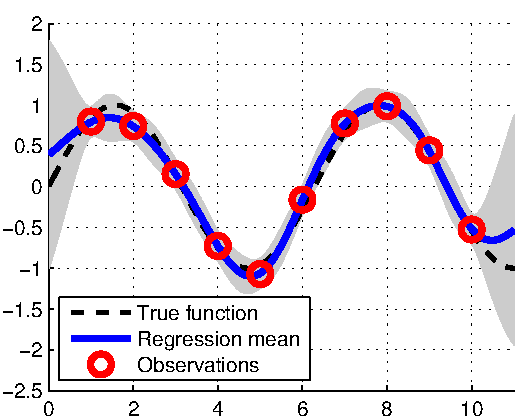
\includegraphics[width=\columnwidth]{reg_ex}
% where an .eps filename suffix will be assumed under latex,
% and a .pdf suffix will be assumed for pdflatex; or what has been declared
% via \DeclareGraphicsExtensions.
\caption{GP regression example (placeholder)}
\label{reg_ex}
\end{figure}


\subsection{GP Regression Solution to Basic LFM Inference}\label{sec:gp:regression:lfm}
%
%\simo{Mauricio writes but Simo will then contribute}

A canonical example of a linear latent force model (LFM) \cite{Alvarez+Lawrence:2009,Alvarez+Luengo+Lawrence:2013} is the following:
%
\begin{eqnarray}
  &u(t) \sim \mathcal{GP}(0,k(t - t')), \label{eq:lgp1} \\
  &a_n \, \frac{df^{n}(t)}{dt^{n}} + \cdots
  + a_1 \, \frac{df(t)}{dt} + a_0 = u(t), \label{eq:difeq1} \\
  &y_k = f(t_k) + \epsilon_k, \label{eq:meas1}
\end{eqnarray}
%
which contains three parts: a Gaussian process part \eqref{eq:lgp1}, a differential equation part \eqref{eq:difeq1}, and a measurement model \eqref{eq:meas1}. 

Equation \eqref{eq:difeq1} can written as $L{f(t)}=u(t)$, where $L$ is a linear
differential operator of the form $L\equiv a_n \, \frac{d}{dt^{n}} + \cdots
  + a_1 \, \frac{d}{dt} + a_0 $. The differential operator $L$ can be related to a so called Green's function or
impulse response $h(t)$.
%\simo{What should we actually put here?}
On the stationary stage the solution to the differential equation \eqref{eq:difeq1} can be expressed as
%
\begin{equation}
\begin{split}
  f(t) &= \int_{-\infty}^{t} h(t - s) \, u(s) \, ds,
\end{split}
\end{equation}
%
where $h(t)$ is the impulse response of the system. When $u(s)$ is a Gaussian process with zero mean and covariance function $k(t - t')$ then we can easily compute the covariance function of the process $f(t)$:
%
\begin{equation}
\begin{split}
  k_{f,f}(t, t') &=
  \int_{-\infty}^{t} \int_{-\infty}^{t'}
  h(t - s) \, h(t' - s') \, k(s - s') \, ds \, ds',
\end{split}
\label{eq:fcov}
\end{equation}
%
Thus we can replace the problem defined by \eqref{eq:difeq1} and \eqref{eq:lgp1} with an equivalent Gaussian process regression problem
%
\begin{eqnarray}
  &f(t) \sim \mathcal{GP}(0,k_{f, f}(t, t')), \label{eq:lgp2} \\
  &y_k = f(t_k) + \epsilon_k. \label{eq:meas2}
\end{eqnarray}
%
We may be interested in computing the predictive distribution for $f(t)$ at a test point $t^*$ given the training samples.
We can then use the GP regression expressions that we saw in section \ref{sec:gp:regression}, where the covariance
function is now given by $k_{f,f}(t,t')$.


We may also be interested in computing the posterior distribution for $u^*$ at a test time point $t^*$ given noisy
measurements $y_1, \ldots, y_n$ at input times $t_1, \ldots, t_n$. To that end, we compute the cross-covariance function
between the input process $u(t)$, and the output process $f(t)$, using
\begin{align}
k_{f,u}(t,t') & = \int_{-\infty}^t h(t-s)\, k(s - t')\, ds.
\label{eq:fucov}
\end{align}
We assume then that $\mathbf{y}$ and $u^*$ are jointly Gaussian distributed, and their distribution follows
\begin{align*}
\begin{pmatrix}
\mathbf{y}\\
u^*
\end{pmatrix}\sim
\mathcal{N}
\left(
\begin{pmatrix}
\mathbf{0}\\
0
\end{pmatrix},
\begin{pmatrix}
\mathbf{K}_{f,f}(\mathbf{t}, \mathbf{t}) + \sigma^2\mathbf{I} & \mathbf{k}_{f,u}(\mathbf{t}, t^*)\\
\mathbf{k}_{f,u}^{\top}(\mathbf{t}, t^*) & k(t^*, t^*),
\end{pmatrix}
\right),
\end{align*}
where $\mathbf{K}_{f,f}(\mathbf{t}, \mathbf{t})\in\mathbb{R}^{n\times n}$ is a matrix with entries given by
$\{k_{f,f}(t_i, t_j)\}_{i=1, j=1}^{n,n}$, and $\mathbf{k}_{f,u}(\mathbf{t}, t^*) \in\mathbb{R}^{n}$ is a vector with entries
given by $\{k_{f,u}(t_i, t^*)\}_{i=1}^{n}$. Notice that due to the assumed independence between $u(t)$ and $\epsilon_k$,
the covariance between the process $y(t)$ and $u(t)$ is the same than the covariance between the process $f(t)$, and
$u(t)$.

Posterior distribution for $u^*$ given $\mathbf{y}$ follows a Gaussian distribution with mean $\mu_{u^*|\mathbf{y}}$, and
variance $\sigma^2_{u^*|\mathbf{y}}$,
\begin{align*}
\mu_{u^*|\mathbf{y}} & = \mathbf{k}_{f,u}^{\top}(t^*, \mathbf{t})\left[\mathbf{K}_{f,f}(\mathbf{t}, \mathbf{t})
+ \sigma^2\mathbf{I}\right]^{-1}\mathbf{y}\\
\sigma^2_{u^*|\mathbf{y}} & =  k(t^*, t^*) - \mathbf{k}_{f,u}^{\top}(\mathbf{t}, t^*)\left[\mathbf{K}_{f,f}(\mathbf{t}, \mathbf{t})
+ \sigma^2\mathbf{I}\right]^{-1}\mathbf{k}_{f,u}(\mathbf{t}, t^*).
\end{align*}

The approach introduced by
\cite{Alvarez+Lawrence:2009,Alvarez+Luengo+Lawrence:2013} conveniently
reduces the original LFM into an Gaussian process regression problem
with a modified covariance function. However, this approach requires
that we need to solve the impulse response $h$ and then compute the
covariance functions via \eqref{eq:fcov}, and \eqref{eq:fucov}.  If we can obtain closed form
expressions for them, then the inference procedure becomes very
easy. Otherwise numerical computations are needed.

%Here, we could explain with a more bit of detail than in the previous section, all the work done together with Neil in the
%context of the Machine learning perspective to construct GPs.

\subsection{Partial Differential Equation Based LFMs}
%
Similar to the case of ordinary differential equations, we can associate a Green's function to a linear partial differential
operator \cite{Myintu:LPDEBook:2006, Polyanin:Handbook02}.\footnote{The presentation here refers to boundary value
problems.}
Let $G(\mathbf{x}, \mathbf{x}')$ be the Green's function for a
particular linear partial differential operator, where $\mathbf{x}\in\mathbb{R}^p$ is a general input vector that could
include different types of input variables. For example, the vector $\mathbf{x}$ could refer to
coordinates $x$ and $y$ for the Laplace equation in two spatial dimensions, or to coordinate $x$ and time
$t$ for the Heat equation in one spatial dimension.

For example
\begin{align*}
  \frac{\partial f(\mathbf{x})}{\partial t} &= \nabla^2 f(\mathbf{x},t) + u(\mathbf{x},t)
\end{align*}
%
\simo{Should change this to Heat equation's green's function:}
Solution for $f(\mathbf{x})$ follows
\begin{align*}
f(\mathbf{x}) & = \int_{\mathcal{X}}G(\mathbf{x},  \mathbf{z})\,
                u(\mathbf{z})\,d\mathbf{z}
%+ g(\mathbf{x}),
\end{align*}
where $\mathcal{X}$ is the input domain of integration, and
$g(\mathbf{x})$ is the solution due to initial and boundary
conditions. For simplicity in the presentation, we assume that the
initial and boundary conditions are zero, but initial and boundary conditions could also be incorporated.

For the GP regression view of latent force models, we put a GP prior over $u(\mathbf{x})$,
\begin{align*}
u(\mathbf{x})\sim\mathcal{GP}(0, k(\mathbf{x} - \mathbf{x}')).
\end{align*}
Covariance for $f(\mathbf{x})$ then follows a similar expression to \eqref{eq:fcov},
\begin{equation}
\begin{split}
  k_{f,f}(\mathbf{x}, \mathbf{x}') &=
  \int_{\mathcal{X}}   \int_{\mathcal{X}}
  G(\mathbf{x}, \mathbf{z}) \, G(\mathbf{x}', \mathbf{z}') \, k(\mathbf{z}, \mathbf{z}') \, d\mathbf{z} \, d\mathbf{z}'.
\end{split}
\notag
%\label{eq:fcov:pde}
\end{equation}
Cross-covariance between the output process $f(\mathbf{x})$, and the input process $u(\mathbf{x})$ can also be computed
using a similar expression to \eqref{eq:fucov}
\begin{align}
k_{f,u}(\mathbf{x},\mathbf{x}') & = \int_{\mathcal{X}} G(\mathbf{x}, \mathbf{z})\, k(\mathbf{z} - \mathbf{x}')\, d\mathbf{z}.
\notag
%\label{eq:fucov}
\end{align}
Based on a set of noisy training samples, $\mathcal{D}=\{\mathbf{x}_k, y_k\}_{k=1}^n$, we can
use the GP regression equations in sections \ref{sec:gp:regression} and \ref{sec:gp:regression:lfm}, to make predictions
for a test input $\mathbf{x}^*$, both for the output process $f(\mathbf{x})$, and the input process $u(\mathbf{x})$.

\simo{Should visualize something on Heat equation here}

\simo{Generalization to any linear PDE}

\simo{Especially non-time-based models such as the Poisson equation.}

\section{Latent Force Models as Stochastic State-Space Models}

\subsection{GPs in state-space form}
As shown in \cite{Hartikainen+Sarkka:2010,Sarkka+Solin+Hartikainen:2013,Sarkka+Piche:2014} many covariance function based models of the form
%
\begin{equation}
  u(t) \sim \mathcal{GP}(0,k(t - t'))
\end{equation}
%
can be equivalently or approximately expressed in state-space form by defining a state vector such as $\mathbf{u} = (u, du/dt,\ldots,d^{p-1}u/dt^{p-1})$---note that depending on parameterization the state vector might not contain exactly the derivatives, but something related---leading to a state-space model
%
\begin{equation}
\begin{split}
  \frac{d\mathbf{u}(t)}{dt}
  &= \mathbf{A}_u \, \mathbf{u}(t) + \mathbf{B}_u \, w(t) \\
  u(t) &= \mathbf{C}_u \, \mathbf{u}(t),
\end{split}
\label{eq:ssu}
\end{equation}
%
where $w(t)$ is a white-noise process. The advantage of this kind of model formulation is that it allows for solving the GP regression problem using Kalman filters and smoothers \cite{Sarkka:2013} in $O(n)$ time when the traditional GP takes $O(n^3)$ time (here $n$ denotes the number of measurements).

The key (classical) result is that such a white-noise-driven state-space representation exists if and only if the spectral density (the Fourier transform of $k(\tau)$) is a proper rational function:
%
\begin{equation}
\begin{split}
  S(\omega) &= \frac{d_0 + d_1 \, \omega^2 + \cdots + d_r \, \omega^{2r}}{c_0 + c_1 \, \omega^2 + \cdots + c_s \, \omega^{2s}}.
\end{split}
\end{equation}
%
By using the spectral factorization and classical state-space realizations \cite{Sarkka+Solin+Hartikainen:2013} it is then possible to construct the matrices $\mathbf{A}_u$, $\mathbf{B}_u$, and $\mathbf{C}_u$ such that $u(t)$ has the desired covariance function. 

For example, the Mat\'ern covariance functions  $k(\tau) = \left( \sigma^2 \, 2^{1-\nu} / \Gamma(\nu)\right) \left(\sqrt{2\nu}\,\tau / \ell \right)^\nu K_\nu\left(\sqrt{2\nu}\,\tau / \ell \right)$ with certain parameter values ($\nu=1/2,3/2,\ldots$) have exact state-space representations. In particular, with $\nu=3/2$ we get
 %
\begin{equation}
\begin{split}
\frac{d\mathbf{u}(t)}{dt} &= \underbrace{\begin{pmatrix} 0 & 1 \\ -\lambda^2 & -2\lambda \end{pmatrix}}_{\mathbf{A}_u}
 \, \mathbf{u}(t)
+ \underbrace{\begin{pmatrix} 0 \\ 1 \end{pmatrix}}_{\mathbf{B}_u} \, w(t), \\
   u(t) &= \underbrace{\begin{pmatrix} 1 & 0 \end{pmatrix}}_{\mathbf{C}_u} \, \mathbf{u}(t),
\end{split}
\end{equation}
%
where $\lambda=\sqrt{2\nu}/\ell$. 

Although the commonly used squared exponential covariance function does not have an exact state-space representation, it can be easily it can be approximated with such using a simple Taylor series expansions or Pad\'e approximants in Fourier domain \cite{Sarkka+Piche:2014}. State-space representations of periodic covariance functions have been considered in \cite{Solin+Sarkka:2014a}, and rational quadratic and general scale mixtures of Gaussians in \cite{Solin+Sarkka:2014b}.

It is also possible to extend this concept to spatio-temporal covariance functions of the form $k(\mathbf{x} - \mathbf{x}', t-t')$, which in turn gives covariance functions $k(\mathbf{x} - \mathbf{x}')$ as a special case, because we can always reinterpret one of the components of $\mathbf{x}$ as time. The methods to form these infinite-dimensional state-space representations have been considered in \cite{Sarkka+Hartikainen:2012,Sarkka+Solin+Hartikainen:2013}. 

The conversion of spatio-temporal covariance function into state-space form leads to a system of the form
%
\begin{equation}
\begin{split}
  \frac{\partial\mathbf{u}(\mathbf{x},t)}{\partial t} &= \mathbf{\mathcal{A}}_u \, \mathbf{u}(\mathbf{x},t)
  + \mathbf{B}_u \, w(\mathbf{x},t) \\
   u(\mathbf{x},t) &= \mathbf{C}_u \, \mathbf{u}(\mathbf{x},t),
\end{split}
\label{eq:ssu2}
\end{equation}
%
where $\mathbf{\mathcal{A}}_u$ is a matrix of linear operators (typically pseudo-differential operators) acting on the $\mathbf{x}$-variable and $w(\mathbf{x},t)$ is a time-white spatio-temporal Gaussian process. This representation can be obtained by an extension the spectral factorization based method for the temporal case. 

For example, the spatio-temporal Mat\'ern covariance function with a suitable parametrization leads to the following representation \cite{Sarkka+Solin+Hartikainen:2013}:
%
\begin{equation}
\begin{split}
  \frac{\partial \mathbf{u}(\mathbf{x},t)}{\partial t} &= 
       \underbrace{\begin{pmatrix} 
        0 & 1 \\ 
        \nabla^2-\lambda^2
        & -2 \sqrt{\lambda^2-\nabla^2} 
      \end{pmatrix}}_{\mathbf{\mathcal{A}}_u} \mathbf{u}(\mathbf{x},t)
      + \underbrace{\begin{pmatrix} 0 \\ 1 \end{pmatrix}}_{\mathbf{B}_u} w(\mathbf{x},t), \\
      u(\mathbf{x},t) &= \underbrace{\begin{pmatrix} 1 & 0 \end{pmatrix}}_{\mathbf{C}_u} \, \mathbf{u}(\mathbf{x},t),
\end{split}
\label{2dmatern_ss}
\end{equation}
%
where $\nabla^2 = \partial^2 / \partial x_1^2 + \cdots + \partial^2 / \partial x_p^2$ and $\sqrt{\cdot}$ in the matrix $\mathbf{\mathcal{A}}_u$ denotes an operator square root.

State-space realizations of spatio-temporal oscillating fields have been discussed in \cite{Solin+Sarkka:2013}. The implementation of divergence-free covariance functions for magnetic field modeling have been recently presented in \cite{Solin:2015}.

\simo{Should add a visualization of this idea here}

\subsection{LFMs in state-space form}
%
We can rewrite the basic LFM differential equation \eqref{eq:difeq1} in state-space form by defining a state vector $\mathbf{f} = (f, df/dt,\ldots,d^{n-1}f/dt^{n-1})$ and writing
%
\begin{equation}
\begin{split}
  \frac{d\mathbf{f}(t)}{dt}
  &= \underbrace{\begin{pmatrix}
       0             & 1      &        &       \\
                     & \ddots & \ddots &       \\
                     &         &  0    &     1 \\
   -a_0 & -a_1 & \hdots &  -a_{n-1}
  \end{pmatrix}}_{\mathbf{A}_f} \, \mathbf{f}(t)
  + \underbrace{\begin{pmatrix}
      0 \\
      \vdots \\
      0 \\
      \frac{1}{a_n}
  \end{pmatrix}}_{\mathbf{B}_f} \,
   u(t) \\
   f(t) &= \underbrace{\begin{pmatrix}
     1 & 0 & \cdots & 0
   \end{pmatrix}}_{\mathbf{C}_f} \, \mathbf{f}(t)
\end{split}
\label{eq:ss1}
\end{equation}
%
This gives the following state-space representation for $f(t)$:
%
\begin{equation}
\begin{split}
  \frac{d\mathbf{f}(t)}{dt}
  &= \mathbf{A}_f \, \mathbf{f}(t) + \mathbf{B}_f \, u(t) \\
  f(t) &= \mathbf{C}_f \, \mathbf{f}(t).
\end{split}
\label{eq:ssgen}
\end{equation}
%
We can now combine the above state-space representation with the state-space representation of LFMs in the previous section to obtain an augmented state-space representation of the LFM \cite{Hartikainen+Sarkka:2011,Hartikainen+Seppanen+Sarkka:2012}. Thus we obtain a combined model
%
\begin{equation}
\begin{split}
  \frac{d\mathbf{f}(t)}{dt}
  &= \mathbf{A}_f \, \mathbf{f}(t)
  + \mathbf{B}_f \, \mathbf{C}_u \, \mathbf{u}(t) \\
  \frac{d\mathbf{u}(t)}{dt}
  &= \mathbf{A}_u \, \mathbf{u}(t) + \mathbf{B}_u \, w(t) \\
  f(t) &= \mathbf{C}_f \, \mathbf{f}(t).
\end{split}
\label{eq:comb}
\end{equation}
%
If we now define
%
\begin{equation}
\begin{split}
  \mathbf{g} &= \begin{pmatrix}
	\mathbf{f} \\ \mathbf{u}
  \end{pmatrix}, \quad
  \mathbf{A}
  = \begin{pmatrix}
	\mathbf{A}_f & \mathbf{\mathbf{B}_f \, \mathbf{C}_u} \\
	0 & \mathbf{A}_u
  \end{pmatrix} \\
  \mathbf{B}
  &= \begin{pmatrix}
	0 & \mathbf{B}_u
  \end{pmatrix}, \quad
  \mathbf{C}
  = \begin{pmatrix}
	\mathbf{C}_f & 0
  \end{pmatrix}
\end{split}
\end{equation}
%
then the model can be written as a white-noise driven state-space model
%
\begin{equation}
\begin{split}
  \frac{d\mathbf{g}(t)}{dt}
  &= \mathbf{A} \, \mathbf{g}(t)
  + \mathbf{B} \, w(t) \\
  f(t) &= \mathbf{C} \, \mathbf{g}(t).
\end{split}
\label{eq:ssaug}
\end{equation}
%
The measurements can be included into the model by replacing the second equation above by
%
\begin{equation}
\begin{split}
  y_k &= \mathbf{C} \, \mathbf{g}(t_k) + \epsilon_k.
\end{split}
\label{eq:ssaugkf}
\end{equation}
%
The advantage of this formulation is that we can infer both the process and the latent Gaussian process via Kalman filtering and smoothing in linear time (see \cite{Hartikainen+Sarkka:2010,Sarkka+Solin+Hartikainen:2013}). The link to Kalman filtering and smoothing follows from the result that as the model above is linear, we can form an exact (error-free) discretization of the model as
%
\begin{equation}
\begin{split}
  \mathbf{g}_k
  &= \mathbf{U}(\Delta t_k) \, \mathbf{g}_{k-1}
  + \mathbf{q}_k \\
  y_k &= \mathbf{C} \, \mathbf{g}_k + \epsilon_k.
\end{split}
\label{eq:dssaug}
\end{equation}
%
where $\mathbf{g}_k \triangleq \mathbf{g}(t_k)$, $\mathbf{q}_k \sim \mathcal{N}(0,\mathbf{Q}(\Delta t_k)$, $\Delta_t = t_k - t_{k-1}$, and
%
\begin{equation}
\begin{split}
  \mathbf{U}(\Delta t_k)  &= \exp(\Delta t_k \, \mathbf{A}), \\
  \mathbf{Q}(\Delta t_k) &= \int_0^{\Delta t_k} \exp((\Delta t_k - \tau) \, \mathbf{A}) \,
  \mathbf{B} \, q_c  \, \mathbf{B}^T \\
  &\qquad \quad \times \exp((\Delta t_k - \tau) \, \mathbf{A})^T \, d\tau,
\end{split}
\label{eq:dssaug}
\end{equation}
%
where $q_c$ is the spectral density of the white noise $w(t)$. For numerical computation of the matrix exponential and the above integral there exists a wide range of numerical methods (see, e.g., \cite{Grewal+Andrews:2001,Sarkka:2006}) with ready-available implementations.

The link to Kalman filtering results from the fact that the model \eqref{eq:dssaug} is a standard discrete-time linear Gaussian model and the Kalman filter and (Rauch--Tung--Striebel, RTS) smoother provide the equations for exact Bayesian inference on it (see, e.g., \cite{Sarkka:2013}). 

\subsection{Partial differential equations in state-space form}
%
Partial differential equation models driven by Gaussian processes can also be often represented in a similar state-space form as the temporal models considered in the previous section. Consider for example the heat equation
%
\begin{equation}
\begin{split}
  \frac{\partial f(\mathbf{x},t)}{\partial t} &=
  D \, \nabla^2 \, f(\mathbf{x},t) - \beta \, f(\mathbf{x},t) + u(\mathbf{x},t) \\
\end{split}
\end{equation}
%
Let us now assume that we are have a state-space representation of the unknown function $u(\mathbf{x},t)$ in form \eqref{eq:ssu2}. This thus leads to the system
%
\begin{equation}
\begin{split}
  \frac{\partial f(\mathbf{x},t)}{\partial t} &=
  \underbrace{\left( D \, \nabla^2 - \beta \right)}_{\mathbf{\mathcal{A}}_f} \, f(\mathbf{x},t) + \mathbf{C}_u \, \mathbf{u}(\mathbf{x},t) \\
  \frac{\partial\mathbf{u}(\mathbf{x},t)}{\partial t} &= \mathbf{\mathcal{A}}_u \, \mathbf{u}(\mathbf{x},t)
  + \mathbf{B}_u \, w(\mathbf{x},t) \\
\end{split}
\end{equation}
%
where the analogy to the model \eqref{eq:comb} is apparent. For higher order derivatives on the left hand side we should define a vector of derivatives $\begin{pmatrix} f, \partial f/\partial t, \ldots \end{pmatrix}$, but for the present first order case this is unnecessary.

In order to obtain a single augmented model, analogously to the previous section we can define (with $\mathbf{B}_f = 1$ in this particular case)
%
\begin{equation}
\begin{split}
  \mathbf{g} &= \begin{pmatrix}
	\mathbf{f} \\ \mathbf{u}
  \end{pmatrix}, \quad
  \mathbf{\mathcal{A}}
  = \begin{pmatrix}
	\mathbf{\mathcal{A}}_f & \mathbf{B}_f \, \mathbf{C}_u \\
	0 & \mathbf{\mathcal{A}}_u
  \end{pmatrix} \\
  \mathbf{B}
  &= \begin{pmatrix}
	0 & \mathbf{B}_u
  \end{pmatrix}, \quad
  \mathbf{C}
  = \begin{pmatrix}
	1 & 0
  \end{pmatrix}
\end{split}
\end{equation}
%
which leads to a model of the form
%
\begin{equation}
\begin{split}
  \frac{\partial \mathbf{g}(\mathbf{x},t)}{\partial t}
  &= \mathbf{\mathcal{A}} \, \mathbf{g}(\mathbf{x},t)
  + \mathbf{B} \, w(\mathbf{x},t) \\
  y_k &= \mathbf{C} \, \mathbf{g}(t_k) + \epsilon_k.
\end{split}
\label{eq:ssaug2}
\end{equation}
%
The discretization now proceeds analogously to the previous section, except that the matrix exponential is replaced with a operator exponential (exponential semigroup) and its time-integral:
%
\begin{equation}
\begin{split}
  \mathbf{\mathcal{U}}(\Delta t_k)  &= \exp(\Delta t_k \, \mathbf{\mathcal{A}}), \\
  \mathbf{Q}(\mathbf{x},\mathbf{x}';\Delta t_k) &= \int_0^{\Delta t_k} \exp((\Delta t_k - \tau) \, 
  \mathbf{\mathcal{A}}) \,
  \mathbf{B} \, q_c(\mathbf{x},\mathbf{x}')  \, \mathbf{B}^T \\
  &\qquad \quad \times \exp((\Delta t_k - \tau) \, \mathbf{\mathcal{A}})^T \, d\tau.
\end{split}
\label{eq:dssaug}
\end{equation}
%
Furthermore, both the spectral density $q_c(\mathbf{x},\mathbf{x}')$ and the covariance $\mathbf{Q}(\mathbf{x},\mathbf{x}';\Delta t_k)$ become kernels in $\mathbf{x},\mathbf{x}'$. Note that above, we need to interpret the operator application from the right as operating onto the variable $\mathbf{x}'$ (cf. \cite{Sarkka+Hartikainen:2012}).

The inference in the above model can be done with infinite-dimensional Kalman filters and RTS smoothers (see, \cite{Sarkka+Hartikainen:2012}). However, in practice we often use some kind of basis function expansion methods to project the equations onto a finite-dimensional sub-space which reduces the filters and smoothers to their finite-dimensional versions.

Sometimes we are interested in partial differential equations without time-dependence, with a prototypical example being the Poisson equation
%
\begin{equation}
\begin{split}
  \nabla^2 f(\mathbf{x}) = u(\mathbf{x})
\end{split}
\end{equation}
%
Although there is no time-variable, we can redefine one of the spatial variables as time $\mathbf{x} \triangleq (\mathbf{x},t)$ which thus leads to the equation
%
\begin{equation}
\begin{split}
  \frac{\partial^2 f(\mathbf{x},t)}{\partial t^2} + \nabla^2 f(\mathbf{x},t) = u(\mathbf{x},t)
\end{split}
\label{ipoisson}
\end{equation}
%
However, this kind of equations without builtin physical time-dependence need to more care than physically time dependent equations as will be illustrated in the following.

It would now be tempting to move the term $\nabla^2 f(\mathbf{x},t)$ to the right hand side and form a state-space form via defining the state as $(\mathbf{f},\partial f/\partial t)$. However, this will not lead to a valid state-space model, because the corresponding operator matrix will not correspond to a time-stable system (cf. \cite{Sarkka+Solin+Hartikainen:2013}). This can be easiest seen by taking the spatial Fourier transform of \eqref{ipoisson} which gives
%
\begin{equation}
\begin{split}
  \frac{\partial^2 \tilde{u}(i \boldmath{\omega}_x,t)}{\partial t^2}
  = \| \boldmath{\omega}_x \|^2 \tilde{u}(i \boldmath{\omega}_x,t) + \tilde{u}(i \boldmath{\omega}_x,t)
\end{split}
\end{equation}
%
which can be seen to correspond to a unstable system.

In order to form a valid state-space model, let us take time-space Fourier transform of \eqref{ipoisson} which gives
%
\begin{equation}
\begin{split}
  (i \omega_t)^2 \, F(i \boldmath{\omega}_x,i \omega_t)
  + \| i \boldmath{\omega}_x \|^2 F(i \boldmath{\omega}_x,i \omega_t)= U(i \boldmath{\omega}_x,i \omega_t)
\end{split}
\end{equation}
%
%
which implies that the spectral density of $f$ has the form
%
\begin{equation}
\begin{split}
  S_f(\boldmath{\omega}_x,\omega_t)
  &= \frac{S_u(\boldmath{\omega}_x,\omega_t)}{\left( (\omega_t)^2 \ + \| \boldmath{\omega}_x \|^2 \right)^2}
\end{split}
\end{equation}
%
which can be refactored with respect to $\omega_t$ to give the stable, statistically equivalent system
%
\begin{equation}
\begin{split}
  \frac{\partial^2 f(\mathbf{x},t)}{\partial t^2}
  + 2 \sqrt{-\nabla^2} \, \frac{\partial f(\mathbf{x},t)}{\partial t} - \nabla^2 f(\mathbf{x},t) = u(\mathbf{x},t)
\end{split}
\label{spoisson}
\end{equation}
%
which has the state-space representation
%
\begin{equation}
\begin{split}
  \frac{\partial \mathbf{f}(\mathbf{x},t)}{\partial t} &= 
       \underbrace{\begin{pmatrix} 
        0 & 1 \\ 
        \nabla^2
        & -2 \sqrt{-\nabla^2} 
      \end{pmatrix}}_{\mathbf{\mathcal{A}}_f} \mathbf{f}(\mathbf{x},t)
      + \underbrace{\begin{pmatrix} 0 \\ 1 \end{pmatrix}}_{\mathbf{B}_f} u(\mathbf{x},t), \\
      f(\mathbf{x},t) &= \underbrace{\begin{pmatrix} 1 & 0 \end{pmatrix}}_{\mathbf{C}_f} \, \mathbf{f}(\mathbf{x},t).
\end{split}
\end{equation}
%
This model is now time-stable and can be augmented with a state-space model for $u$ in order to yield a state-space representation for the full LFM model.

%
%\subsection{Discussion or comparison of both approaches}
%
%Maybe here we should give some analysical/numerical examples, making comparisons in terms of the types of covariance function one can get in both methods, or the type of power spectrum one may get. We could also discuss the possibilities to combine with other methods in GP/Kalman areas.

\section{Numerical methods for LFMs}

\subsection{PDE Methods for Covariance Function Computation}
%
One commonly used method for approximate solution of partial differential equations (PDEs) is the Galerkin's method which approximates the solution on a finite-dimensional space spanned by certain basis functions $\{ \phi_i(\mathbf{x})~i=1,2,\ldots,N \}$. With a suitable selection of basis functions it (in its weak formulation) leads to widely-used methods such as finite element method (FEM). As an example, let us consider the Gaussian process driven Poisson equation
%
\begin{equation}
\begin{split}
  \nabla^2 f(\mathbf{x}) = u(\mathbf{x})
\end{split}
\end{equation}
%
Let us now assume, for example, that we are working in a compact subspace $\Omega \subset \mathbb{R}^p$ and define a Hilbert space with an inner product $\langle \cdot, \cdot \rangle$ such that $\{ \phi_i(\mathbf{x})~i=1,2,\ldots,N \}$ are orthonormal with respect to the inner product. We can now approximate $f$ and $u$ via the series expansions
%
\begin{equation}
\begin{split}
   f(\mathbf{x}) &= \sum_{i=1}^N f_i \, \phi_i(\mathbf{x}) \\
   u(\mathbf{x}) &= \sum_{i=1}^N u_i \, \phi_i(\mathbf{x}) \\   
\end{split}
\end{equation}


\simo{Discuss the use of Hilbert-space methods, FEM, and finite differences to approximate the covariance function computation for LFMs both in covariance and state-space form}

\subsection{Matrix and Operator Exponential Computation of Green's Functions}
%
Assume that we have a basic (differential equation) based LFM which has the state-space representation
%
\begin{equation}
\begin{split}
  \frac{d\mathbf{f}(t)}{dt}
  &= \mathbf{A}_f \, \mathbf{f}(t) + \mathbf{B}_f \, u(t) \\
\end{split}
\end{equation}
%
with the function of interest being $f(t) = \mathbf{C}_f \, \mathbf{f}(t)$. Because this system is of the first order, the impulse response can be written down explicitly in terms of the matrix exponential function $\mathbf{U}(t) = \exp(t \, \mathbf{A})$ and hence the joint covariance function of $\mathbf{f}$ is
%
\begin{equation}
\begin{split}
  &\mathbf{K}_\mathbf{f}(t - t')
  \\ &
  =
  \int_{-\infty}^{t} \int_{-\infty}^{t'}
  \mathbf{U}(t - s) \, \mathbf{B}_f \, k(s - s') \,
  \mathbf{B}_f^T \, \mathbf{U}^T(t' - s') \, ds \, ds',
\end{split}
\label{eq:vfcov}
\end{equation}
%
and we can pick up the covariance function of $f(t)$ from the matrix via
%
\begin{equation}
\begin{split}
  k_f(t,t') &=
  \mathbf{C}_f \, \mathbf{K}_\mathbf{f}(t - t') \, \mathbf{C}_f^T
\end{split}
\label{eq:fcov2}
\end{equation}
%
This representation has the advantage that it is easy to numerically approximate the matrix exponential and hence the analytical computation of the impulse response becomes unnecessary. However, we still need to compute the integrals in \eqref{eq:vfcov} somehow. If closed form solution is not available (which surpricing often is), then the computations need to be done via numerical integration.

\simo{If I recall right, we can use the stationarity to reduce this into a single integral, need to check}

For the case of spatio-temporal covariance functions we now get an analogous results, except that matrices are generalized to operators. Assume that that out LFM has the form
%
\begin{equation}
\begin{split}
  \frac{\partial \mathbf{f}(\mathbf{x},t)}{\partial t}
  &= \mathbf{\mathcal{A}}_f \, \mathbf{f}(\mathbf{x},t) + \mathbf{B}_f \, u(\mathbf{x},t) \\
\end{split}
\end{equation}
%
where $\mathbf{\mathcal{A}}_f$ is a matrix of linear operators. Let the covariance function of $u$ be $k(\mathbf{x},\mathbf{x}';t - t')$. Then, if we define the operator exponential $\mathbf{\mathcal{U}}(t) = \exp(t \, \mathbf{\mathcal{A}})$, the covariance function of $f$ can be expressed as
%
\begin{equation}
\begin{split}
  k_f(\mathbf{x},\mathbf{x}';t-t') &=
  \mathbf{C}_f \, \mathbf{K}_\mathbf{f}(\mathbf{x},\mathbf{x}';t-t') \, \mathbf{C}_f^T
\end{split}
\end{equation}
%
with
%
\begin{equation}
\begin{split}
  &\mathbf{K}_\mathbf{f}(\mathbf{x},\mathbf{x}';t-t')
  \\ &
  =
  \int_{-\infty}^{t} \int_{-\infty}^{t'}
  \mathbf{\mathcal{U}}(t - s) \, \mathbf{B}_f \, k(\mathbf{x},\mathbf{x}';s - s') \,
  \mathbf{B}_f^T \, \mathbf{\mathcal{U}}^T(t' - s') \, ds \, ds',
\end{split}
\label{eq:vfcov}
\end{equation}
%
where the operator multiplication from right is again interpreted as acting onto the variable $\mathbf{x}'$.

\simo{Some more text to follow especially in relation to numerical methods in previous section.}

\subsection{Separable Covariance Functions}
%
\simo{Some tips and tricks for separable covariance functions.}

\subsection{Stable State-Space Realization of $u$}
%
In this section we discuss stable representation of the rational spectral densities needed to $u$. Recall that the first step in the construction of the state-space model is spectral factorization (see, e.g., \cite{Hartikainen+Sarkka:2010, Sarkka+Hartikainen:2012, Sarkka+Solin+Hartikainen:2013}) which means that given a rational spectral density $S(\omega)$, we find a real rational function
%
\begin{equation}
\begin{split}
 G(i \, \omega)
 = \frac{\tilde{b}_m \, (i \, \omega)^m + \tilde{b}_{m-1} \, (i \, \omega)^{m-1} + \cdots
   \tilde{b}_1 \, (i \, \omega) + \tilde{b}_0}
   {(i \, \omega)^n + \tilde{a}_{n-1} \, (i \, \omega)^{n-1} + \cdots + \tilde{a}_1 \, (i \, \omega) + \tilde{a}_0}
\end{split}
\label{eq:trans2}
\end{equation}
%\begin{equation}
%\begin{split}
%  G(s)
%  = \frac{\tilde{b}_m \, s^m + \tilde{b}_{m-1} \, s^{m-1} + \cdots
%    \tilde{b}_1 \, s + \tilde{b}_0}
%    {s^n + \tilde{a}_{n-1} \, s^{n-1} + \cdots + \tilde{a}_1 \, s + \tilde{a}_0}
%\end{split}
%\label{eq:trans2}
%\end{equation}
%
which is analytic and non-zero in the right half plane such that
%
\begin{equation}
\begin{split}
  S(\omega) = G(i \, \omega) \, q_c \, G(-i \, \omega),
\end{split}
\end{equation}
%
where $q_c > 0$ is a constant. In practice, a viable way to find the function is by computing the roots of numerator and denominator, which appear in conjugate pairs, and construct $G(i \, omega)$ from the roots having positive imaginary parts. However, many other spectral factorization methods exist as well \cite{Ref-to-spec-fact-survey}.

Given the function $G$ we can then use, for example, the following controllable canonical form (e.g., \cite{Glad+Ljung:2000}) to construct the state-space model (here $q_c$ becomes the spectral density of the white noise process $w(t)$):
%
\begin{equation}
\begin{split}
  \frac{d\mathbf{u}(t)}{dt}
  &= \underbrace{\begin{pmatrix}
       0             & 1      &        &       \\
                     & \ddots & \ddots &       \\
                     &         &  0    &     1 \\
   -\tilde{a}_0 & -\tilde{a}_1 & \hdots &  -\tilde{a}_{n-1}
  \end{pmatrix}}_{\mathbf{A}_u} \, \mathbf{u}(t) 
  + \underbrace{\begin{pmatrix}
      0 \\
      \vdots \\
      0 \\
      1
  \end{pmatrix}}_{\mathbf{L}_u} \,
   w(t) \\
   u(t) &=
   \underbrace{\begin{pmatrix} \tilde{b}_0 & \tilde{b}_1 & \cdots & \tilde{b}_m & 0 & \cdots & 0
   \end{pmatrix}}_{\mathbf{C}_u} \, \mathbf{u}(t),
\end{split}
\end{equation}
%
or alternatively the observable canonical form
%
\begin{equation}
\begin{split}
  \frac{d\mathbf{u}(t)}{dt}
  &= \underbrace{\begin{pmatrix}
       0             &        &        & -\tilde{a}_0 \\
       1             & \ddots &        & -\tilde{a}_1 \\
                     & \ddots &  0     & \vdots   \\
                     &        &  1     & -\tilde{a}_{n-1} \\
  \end{pmatrix}}_{\mathbf{A}_u} \, \mathbf{u}(t) 
  + \underbrace{\begin{pmatrix}
      \tilde{b}_0 \\
      \vdots \\
      \tilde{b}_m \\
      0 \\
      \vdots \\
      0
  \end{pmatrix}}_{\mathbf{L}_u} \,
   w(t) \\
   u(t) &=
   \underbrace{\begin{pmatrix} 0 & \cdots & 0 & 1 \end{pmatrix}}_{\mathbf{C}_u} \, \mathbf{u}(t)
\end{split}
\end{equation}

However, it is important to point out that the direct use of this procedure might result in a numerically unstable model especially when the approximation order is high. To overcome this problem it is often advisable to use the following method. 
Because the choice of state-variable coordinate system is arbitrary, we can define a new process via $\tilde{\mathbf{u}}(t) = \mathbf{T}^{-1} \, \mathbf{u}(t)$, where $\mathbf{T}$ is a constant invertible matrix, to get a new system
%
\begin{equation}
\begin{split}
    \frac{d\tilde{\mathbf{u}}(t)}{dt}
    &= \mathbf{T}^{-1} \, \mathbf{A}_u \, \mathbf{T} \, \tilde{\mathbf{u}}(t)
    + \mathbf{T}^{-1} \, \mathbf{L} \, w(t), \\
   u(t) &= \mathbf{H} \, \mathbf{T} \, \tilde{\mathbf{u}}(t)
\end{split}
\end{equation}
%
which is equivalent to the model \eqref{eq:ssmodel} in (statistical) input-output sense. It can be observed that the numerical stability is essentially governed by the condition number of the matrix $\mathbf{A}_u$. To convert a state-space model with a badly conditioned matrix $\mathbf{A}_u$ into an equivalent model with a well-conditioned matrix we can use the well-known matrix balancing procedure
%\cite{Parlett+Reinsch:1969,Parlett+Reinsch:1971}
\cite{Parlett+Reinsch:1971}
originally developed for numerically stabilizing the computation the eigenvalues of a matrix (implemented, e.g., as the ``balance'' function in Matlab). This procedure gives us a suitable matrix $\mathbf{T}$ which can be used in the transformation above to give a numerically stable state-space model.

\subsection{Covariance Computation via State-Space Representation}
%
\simo{One way to compute the covariance function $k_f$ is to form the state-spate representation of the full system and then use the state-space formula for the covariance.}



\section{Hyperparameter Learning}
%
\subsection{Hyperparameter Learning in Covariance Function Based LFMs}

\subsection{Hyperparameter Learning in State-Space LFMs}


\section{Extensions}

\subsection{Cascaded LFMs}

In cascaded latent force models, we have two non-homogeneous ordinary differential equations acting in a serial way:
the output of the first differential equation is used as the input for the second differential equation
\cite{Honkela:PNAS10}. If $L_1p(t) = u(t)$, refers to the first differential equation,
where $u(t)$ is the input and $p(t)$ is the output, then for the second differential equation we have $L_2f(t) = p(t)$,
where $L_1$ and $L_2$ are both differential operators as before. In \cite{Honkela:PNAS10}, the authors assign a
GP prior to $u(t)$, and find the posterior for $u(t)$, and $p(t)$, which can be computed analytically when $L_1$ and $L_2$
are both differential operators associated to a first order ODE.

\simo{[In wrong place:] In \cite{Gao:latent08}, the process $u(t)$ follows
a GP that is transformed non-linearly before serving as the input for the first ODE. Posterior distributions are
approximated using the MAP-Laplace method. For the same setup, the authors in \cite{Titsias:BMC:2012} use MCMC to
approximate the posterior distributions for the processes involved.}


\simo{Both write}

\subsection{Non-linear Models}

When the input force is modelled as a non-linear transformation of a Gaussian process \cite{Lawrence:gpsim2007a,
Gao:latent08, Titsias:BMC:2012}, it is necessary to resort to an approximation in order to compute the posterior
distribution for $u^*$ given $\mathbf{y}$, or the predictive distribution for $f^*$ given $\mathbf{y}$.

The setup is again an ordinary differential equation of the form $Lf(t)=g(u(t))$, where $g(\cdot)$ is a non-linear function
of the argument. In \cite{Lawrence:gpsim2007a, Gao:latent08}, the authors suggest the MAP-Laplace method
\cite{Bishop:PRML06} as a way to approximate the posterior distribution for $u(t)$. The MAP-Laplace method approximates
the posterior distribution by a
Gaussian distribution centered at the Maximum a Posteriori (MAP) solution. The method implies functional derivatives of the
log-likelihood for computing the gradient and the Hessian that are necessary in the optimization procedure. Functional
derivatives for the terms involved are then computed on a grid using Riemann quadrature. In \cite{Titsias:BMC:2012}, the
authors provide a Markov Chain Monte Carlo (MCMC) procedure to compute the posterior distribution for $u(t)$, as well
as posterior distributions for any parameters appearing as part of the impulse response.

\mauricio{We could go into more details here if we want. I was checking previous published papers and this is really
the only non-linear model that has been proposed before, in the context of LFMs for regression. The non-linearity in the
differential equation has not been published before}.


\simo{Non-linear models in state-space form here}


\subsection{Switching LFMs}

In the basic LFM, the input process $u(t)$ is a continuous process. An important extension in different applied scenarios
is to allow the input force $u(t)$ to be discontinuous. Equally important is to allow the coefficients $\{a_i\}_{i=0}^n$ that
define the differential operator $L$, to take discrete values as function of $t$. The setup now includes a sequential
series of basic LFMs $\{L_jf(t) = u_j(t)\}_{j=1}^J$, each of them applied in a particular time interval
$\{[T_{j-1}, T_j]\}_{j=1}^J$, where $J$ is the maximum number of time intervals considered, $L_j$ is a differential operator
with coefficients $\{a_i^j\}_{i=0,j=1}^{n, J}$, and $\{u_j(t)\}_{j=1}^J$ are GPs with covariance functions $k_j(t,t')$.
Continuity in the output $f(t)$ is ensured by forcing the initial conditions for the $j$-th ODE to take the same value
than the output $f(t)$ and its derivatives, at the last input point for the $j-1$-th time interval.
In \cite{Alvarez:switched11}, the authors use second order differential operators for $L_j$, to sequentially segment
basic movements (also known as motor primitives) from a multivariate time series coming from a robot arm playing table
tennis.

\mauricio{I just realized we should define a letter for the number of datapoints. I was using little n, but now I see
that little n it's been used for the order of the differential operator}

\simo{Both write}

\subsection{Controlled LFMs}
%
\simo{We could also discuss the use of LFMs in control. The state-space representation allows for the use of classical LQ-control theory for this. As the latent forces are modeled as stationary GPs, it implies that the model will not be controllable (from the force), but certainly it will be stabilizable. }

\subsection{\simo{\st{Periodic Latent Functions}}}

\simo{Is this really an extension -- this is anyway a linear LFM? Let's leave this out.}

%\simo{Both write}

%\simo{Take the covariance series expansions from paper by Arno and Simo}

\mauricio{Not sure what to put here, since we haven't really done any periodic latent function applications in the GP
regression context}


\section{Experimental Results}

\subsection{An ODE Model}
%
\simo{Simple spring model with RBF. Compare the computational complexities and easiness of implementation.}

\simo{Mauricio starts by explaining the setup.}

\begin{figure}[!t]
\centering
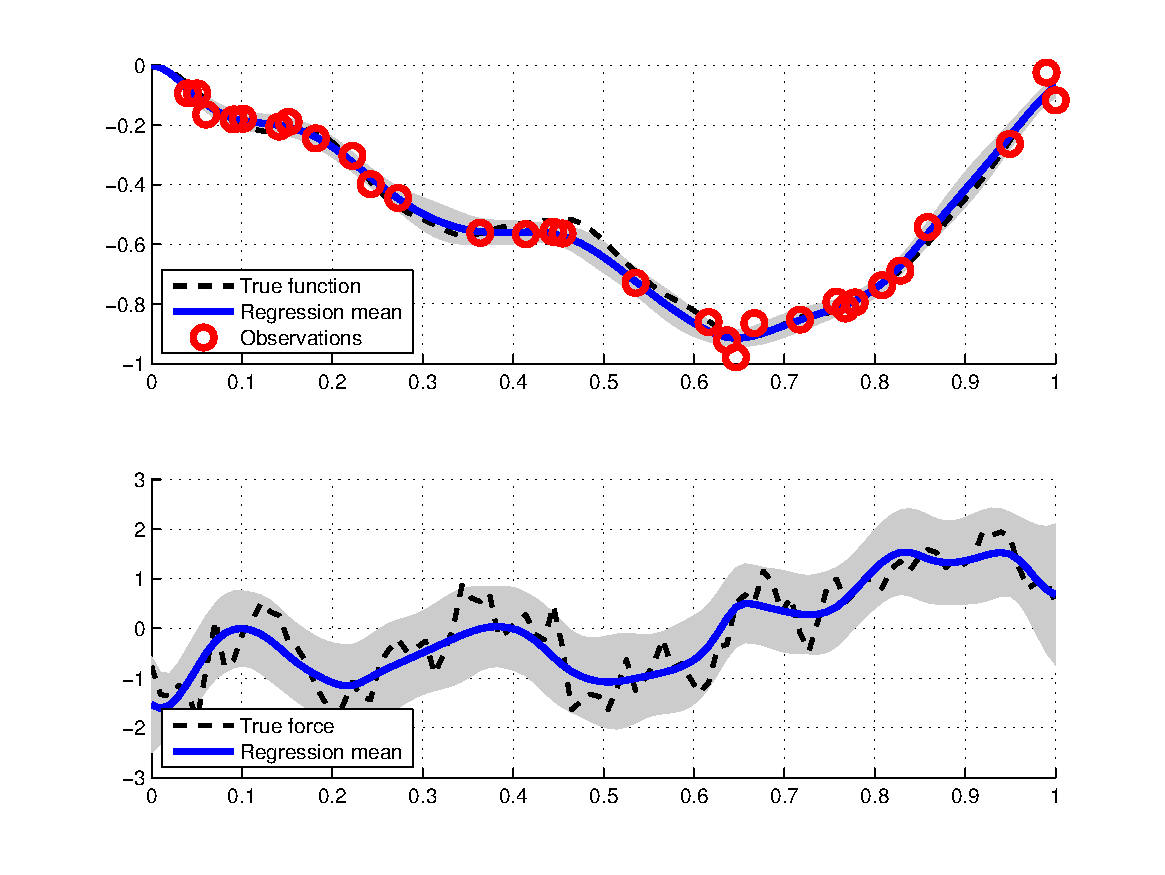
\includegraphics[width=\columnwidth]{placeholder1}
% where an .eps filename suffix will be assumed under latex,
% and a .pdf suffix will be assumed for pdflatex; or what has been declared
% via \DeclareGraphicsExtensions.
\caption{Simulation Results (placeholder 1)}
\label{fig_sim}
\end{figure}


\subsection{A PDE Model}
%
\simo{Heat equation with closed form Green's function and basis functions. Covariance functions RBF \& Matern.}

\simo{Mauricio starts by explaining the setup.}

\begin{figure}[!t]
\centering
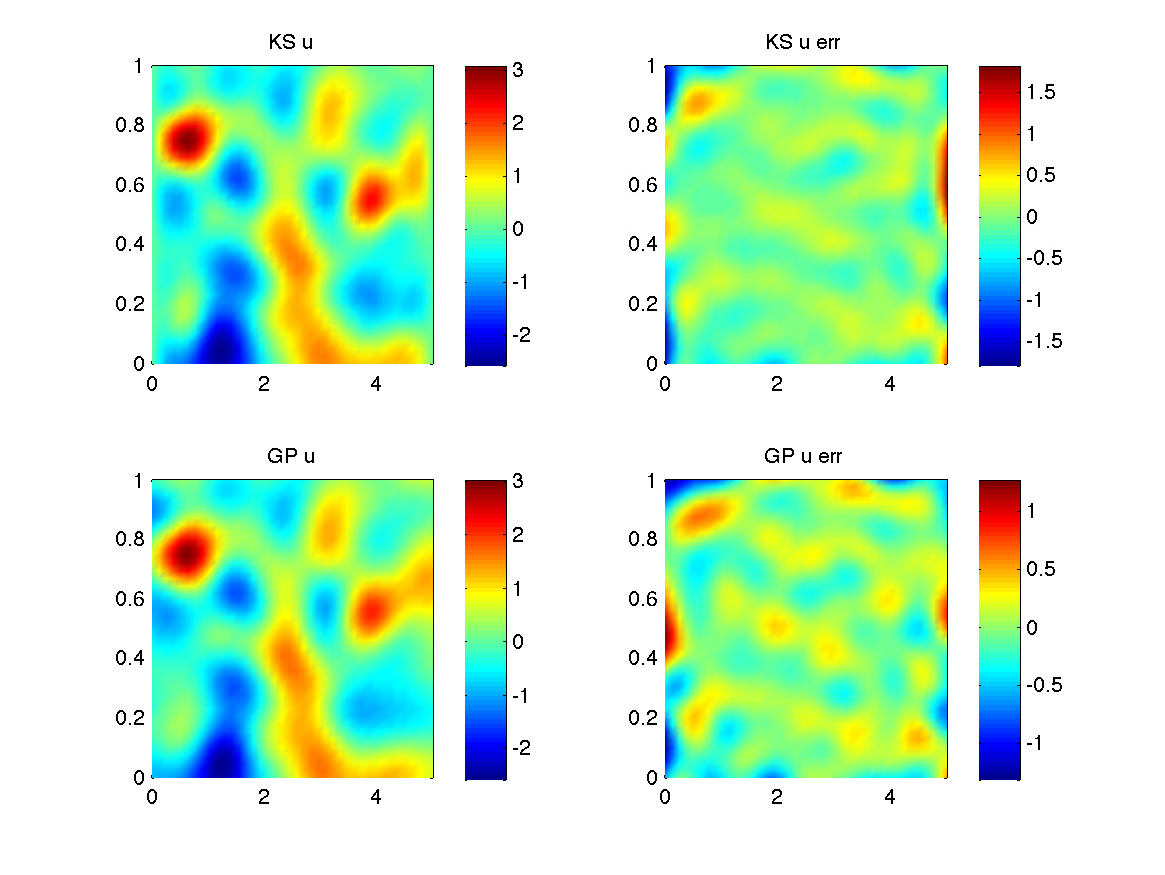
\includegraphics[width=\columnwidth]{placeholder2}
% where an .eps filename suffix will be assumed under latex,
% and a .pdf suffix will be assumed for pdflatex; or what has been declared
% via \DeclareGraphicsExtensions.
\caption{Simulation Results (placeholder 2)}
\label{fig_sim}
\end{figure}

\subsection{A PDE Model II}

\simo{Mauricio writes the Poisson 2D example here, Simo writes the corresponding state-space version. This leads to an interesting (weak) pseudo-differential equation representation of the Poisson model:}

\begin{equation}
\begin{split}
    \frac{\partial\mathbf{u}(\mathbf{x},t)}{\partial t} &= \mathbf{\mathcal{A}}_u \, \mathbf{u}(\mathbf{x},t)
  + \mathbf{B}_u \, w(\mathbf{x},t) \\
  \frac{\partial \mathbf{f}(\mathbf{x},t)}{\partial t} &= 
       \begin{pmatrix} 
        0 & 1 \\ 
        \frac{\partial^2}{\partial x^2}
        & -2 \sqrt{-\frac{\partial^2}{\partial x^2}} 
      \end{pmatrix}\mathbf{u}(\mathbf{x},t)
      + \begin{pmatrix} 0 \\ 1 \end{pmatrix} \mathbf{C}_u \, \mathbf{u}(\mathbf{x},t), \\
      f(\mathbf{x},t) &= \begin{pmatrix} 1 & 0 \end{pmatrix} \, \mathbf{f}(\mathbf{x},t),
\end{split}
\end{equation}

\subsection{LQ Control of LFMs}

%\subsection{\simo{\st{A Periodic Model}}}

%\simo{Probably leave this out}

\section{Conclusions}
The conclusion goes here.





% if have a single appendix:
%\appendix[Proof of the Zonklar Equations]
% or
%\appendix  % for no appendix heading
% do not use \section anymore after \appendix, only \section*
% is possibly needed

% use appendices with more than one appendix
% then use \section to start each appendix
% you must declare a \section before using any
% \subsection or using \label (\appendices by itself
% starts a section numbered zero.)
%


\appendices
\section{Proof of the First Zonklar Equation}
Appendix one text goes here.

% you can choose not to have a title for an appendix
% if you want by leaving the argument blank
\section{}
Appendix two text goes here.


% use section* for acknowledgment
\section*{Acknowledgment}


The authors would like to thank...


% Can use something like this to put references on a page
% by themselves when using endfloat and the captionsoff option.
\ifCLASSOPTIONcaptionsoff
  \newpage
\fi



% trigger a \newpage just before the given reference
% number - used to balance the columns on the last page
% adjust value as needed - may need to be readjusted if
% the document is modified later
%\IEEEtriggeratref{8}
% The "triggered" command can be changed if desired:
%\IEEEtriggercmd{\enlargethispage{-5in}}

% references section

% can use a bibliography generated by BibTeX as a .bbl file
% BibTeX documentation can be easily obtained at:
% http://mirror.ctan.org/biblio/bibtex/contrib/doc/
% The IEEEtran BibTeX style support page is at:
% http://www.michaelshell.org/tex/ieeetran/bibtex/
\bibliographystyle{IEEEtran}
% argument is your BibTeX string definitions and bibliography database(s)
\bibliography{reviewlfm}
%
% <OR> manually copy in the resultant .bbl file
% set second argument of \begin to the number of references
% (used to reserve space for the reference number labels box)
%\begin{thebibliography}{1}

%\bibitem{IEEEhowto:kopka}
%H.~Kopka and P.~W. Daly, \emph{A Guide to \LaTeX}, 3rd~ed.\hskip 1em plus
 % 0.5em minus 0.4em\relax Harlow, England: Addison-Wesley, 1999.
%
%\end{thebibliography}

% biography section
% 
% If you have an EPS/PDF photo (graphicx package needed) extra braces are
% needed around the contents of the optional argument to biography to prevent
% the LaTeX parser from getting confused when it sees the complicated
% \includegraphics command within an optional argument. (You could create
% your own custom macro containing the \includegraphics command to make things
% simpler here.)
%\begin{IEEEbiography}[{\includegraphics[width=1in,height=1.25in,clip,keepaspectratio]{mshell}}]{Michael Shell}
% or if you just want to reserve a space for a photo:

\begin{IEEEbiography}{Michael Shell}
Biography text here.
\end{IEEEbiography}

% if you will not have a photo at all:
\begin{IEEEbiographynophoto}{John Doe}
Biography text here.
\end{IEEEbiographynophoto}

% insert where needed to balance the two columns on the last page with
% biographies
%\newpage

\begin{IEEEbiographynophoto}{Jane Doe}
Biography text here.
\end{IEEEbiographynophoto}

% You can push biographies down or up by placing
% a \vfill before or after them. The appropriate
% use of \vfill depends on what kind of text is
% on the last page and whether or not the columns
% are being equalized.

%\vfill

% Can be used to pull up biographies so that the bottom of the last one
% is flush with the other column.
%\enlargethispage{-5in}



% that's all folks
\end{document}


